\newpage
\subsection{Log Messages}
\subsubsection{Ausgangslage}
Beim Klick auf den Toogle Button, der eine Verbindung zu starten versucht, löst der Webbrowser eine Ajax Request zum Server aus. Dieser blockierende Aufruf lädt die Verbindungskonfiguration in das VICI Interface, startet diese und wartet dann auf Log Messages. Dieser Vorgang kann mehrere Minuten dauern.


\subsubsection{Problematik}
Der Webbrowser möchte möglichst in Echtzeit an diese Loginformationen. Eine mehrere Minuten dauernde Wartezeit (Freeze) kann dem Benutzer nicht zugemutet werden.

\subsubsection{Lösungsansatz}
Die Lösung des Problems bietet die Aufsplittung in zwei verschiedene Ajax Requests. Der erste Request startet die Verbindung und persistiert die empfangenen Log Messages in die Datenbank. Dies Aufruf dauert weiterhin bis zu mehrere Minuten.

Der zweite Request dient der Aktualisierung der Oberfläche, respektive der Anzeige der Log Messages.
Beim Aufruf der Connections Seite wird dieser HTTP Long Polling Request ausgelöst, der die neusten Log Messages zurück gibt. Dieser Request wird dauernd wiederholt, um die Logs auf dem neusten Stand zu halten. Log Messages älter als 5 Minuten werden aus der Datenbank gelöscht. \\
\begin{figure}[H]
\centering
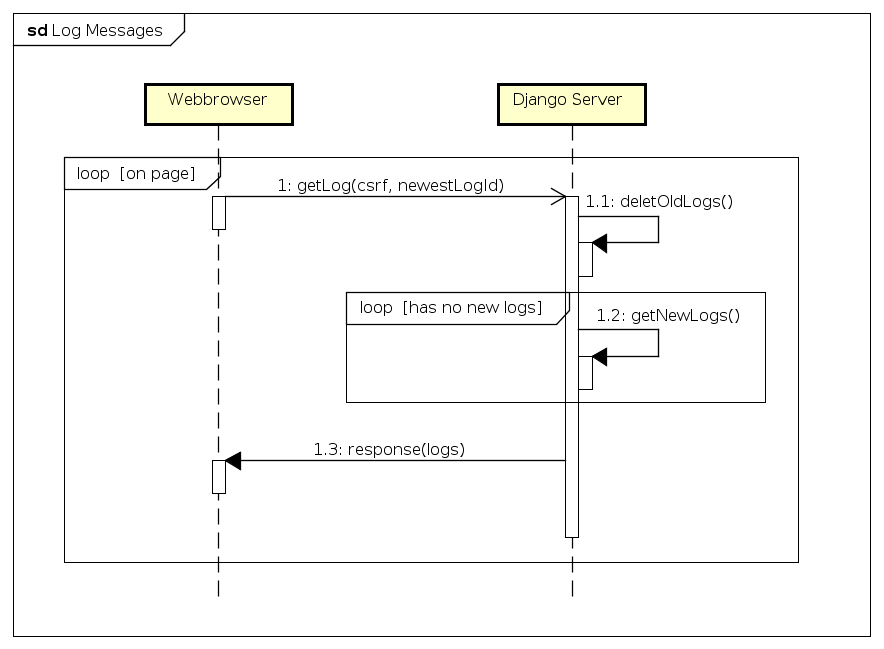
\includegraphics[width=360pt]{images/log_messages_seq.png}
\caption[Log Messages Sequenzdiagramm]{Log Messages Sequenzdiagramm}
\end{figure}